\documentclass[a4paper,12pt]{article}
\usepackage[utf8]{inputenc}
\usepackage{polski}
\usepackage{geometry}
\geometry{margin=2.5cm}
\usepackage{array}
\usepackage{makecell}
\usepackage{amsmath}
\usepackage{siunitx}
\usepackage{graphicx}
\usepackage{float}
\usepackage{subcaption}

\begin{document}

\begin{center}
    \renewcommand{\arraystretch}{1.2}
    \begin{tabular}{|>{\raggedright\arraybackslash}p{9.5cm}|>{\raggedright\arraybackslash}p{5.5cm}|}
        \hline
        \makecell[l]{\textbf{Wydział Informatyki} \\
        Katedra Mediów Cyfrowych i Grafiki Komputerowej \\
        Laboratorium Podstaw Elektrotechniki i Elektroniki}
        &
        \textbf{Data:} 20.05.2025 \\
        \hline
        \makecell[l]{\textbf{Ćwiczenie nr:} 4 \\
        \textbf{Temat:} Diodowe układy prostownicze \\
        \textbf{Grupa:} LAB 9 \\
        \textbf{Imię i nazwisko:} \\
        Wojciech Cimochowski \\
        Radosław Janczura \\
        Kamil Kubajewski}
        &
        \makecell[l]{\textbf{Prowadzący:} \\
        mgr inż. Daniel Grabowski} \\
        \hline
    \end{tabular}
\end{center}
\section*{1. Cel ćwiczeń}

Celem ćwiczeń jest zapoznanie z diodowymi układami prostowniczymi, takimi jak: prostownik jednopołówkowy, prostownik dwupołówkowy z odczepem środkowym oraz prostownik mostkowy. Należy również sprawdzić, jakie będzie napięcie wyjściowe oraz sprawność układu prostownika.

\section*{2. Realizacja ćwiczeń}

Do wykonania zadań użyto modułu AB09 zasilanego napięciem zmiennym sinusoidalnym o wartości 5V i częstotliwości 50Hz. Pomiary wykonano zgodnie z treścią zadań. Użyto oscyloskopu.
\begin{figure}[h]
    \centering
    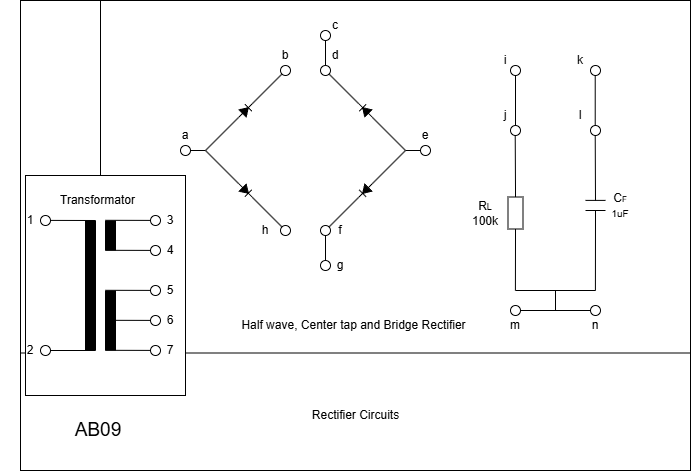
\includegraphics[width=0.8\textwidth]{AB09.png}
    \caption{Schemat obwodu - moduł AB09.}
    \label{fig:schemat}
\end{figure}
\begin{figure}[h]
    \centering
    \includegraphics[width=0.8\textwidth]{1.png}
    \caption{Odczyt z oscyloskopu - wejście.}
    \label{fig:schemat}
\end{figure}
\section*{2.1 Prostownik jednopołówkowy}
Prostownik jednopołówkowy to rzeczywiście najprostsza konfiguracja prostownika, która służy do przekształcania napięcia przemiennego (AC) na napięcie pulsujące stałe (DC). Jego działanie opiera się na wykorzystaniu zaledwie jednej diody półprzewodnikowej, która działa jak jednokierunkowy zawór dla prądu elektrycznego.
\begin{figure}[h]
    \centering
    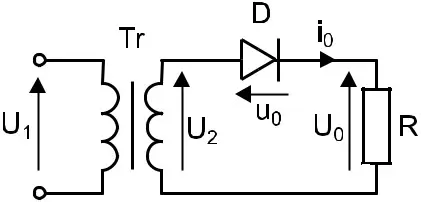
\includegraphics[width=0.8\textwidth]{2.png}
    \caption{Schemat prostownika jednopołówkowego.}
    \label{fig:schemat}
\end{figure}
\section*{Wyniki i obliczenia}

\subsection*{Pomiar}


\begin{itemize}
    \item \textbf{Bez kondensatora:} zakres napięcia: 0 -- 900 mV
    \item \textbf{Z kondensatorem:} napięcie stabilizowane w zakresie 680 -- 840 mV
\end{itemize}
\begin{figure}[h]
    \centering
    \begin{subfigure}{0.45\textwidth}
        \centering
        \includegraphics[width=\linewidth]{3.png}
        \caption{Odczyt pomiaru bez kondensatora.}
        \label{fig:schemat1}
    \end{subfigure}
    \hfill
    \begin{subfigure}{0.45\textwidth}
        \centering
        \includegraphics[width=\linewidth]{4.png}
        \caption{Odczyt pomiaru z kondensatorem.}
        \label{fig:schemat2}
    \end{subfigure}
    \caption{Porównanie odczytów z oraz bez kondensatora.}
    \label{fig:porownanie}
\end{figure}

\subsection*{Teoretyczne obliczenia}
\[
P_{dc} = I_{dc}^2 \cdot R_L = \left( \frac{I_m}{\pi} \right)^2 \cdot R_L
\]

\[
P_{ac} = I_{rms}^2 \cdot (r_f + R_L), \quad \text{gdzie } I_{rms} = \frac{I_m}{2}
\]

gdzie $r_f$ jest rezystancją diody, na stronie producenta podane $0{,}6\ \Omega$, w naszych obliczeniach przyjmiemy $1\ \Omega$.


\subsection*{Obliczona sprawność}

\[
\eta = \frac{P_{dc}}{P_{ac}} \cdot 100\% = 0{,}406 \left( 1 + \frac{r_f}{R_L} \right) \cdot 100\% = 0{,}406 \left( 1 + \frac{1\,\Omega}{100000\,\Omega} \right) \cdot 100\% \approx 40{,}6\%
\]

\section*{2.2 Prostownik dwupołówkowy z odczepem środkowym}

Prostownik dwupołówkowy z odczepem środkowym wykorzystuje dwie diody i transformator z odczepem środkowym. Umożliwia to przewodzenie prądu w obu połówkach cyklu napięcia przemiennego, co skutkuje mniejszymi tętnieniami i wyższą sprawnością w porównaniu z prostownikiem jednopołówkowym.

\begin{figure}[H]
    \centering
    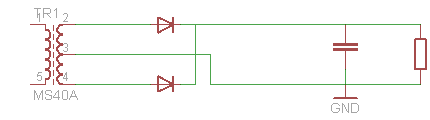
\includegraphics[width=0.8\textwidth]{5.png}
    \caption{Schemat prostownika dwupołówkowego z odczepem środkowym.}
    \label{fig:schemat_dwu}
\end{figure}

\section*{Wyniki i obliczenia}

\subsection*{Pomiar}

\begin{itemize}
    \item \textbf{Bez kondensatora:} napięcie wyjściowe: 0 -- 832 mV
    \item \textbf{Z kondensatorem:} napięcie: 696 -- 784 mV
\end{itemize}
\begin{figure}[h]
    \centering
    \begin{subfigure}{0.45\textwidth}
        \centering
        \includegraphics[width=\linewidth]{6.png}
        \caption{Odczyt pomiaru bez kondensatora.}
        \label{fig:schemat1}
    \end{subfigure}
    \hfill
    \begin{subfigure}{0.45\textwidth}
        \centering
        \includegraphics[width=\linewidth]{7.png}
        \caption{Odczyt pomiaru z kondensatorem.}
        \label{fig:schemat2}
    \end{subfigure}
    \caption{Porównanie odczytów z oraz bez kondensatora.}
    \label{fig:porownanie}
\end{figure}
\subsection*{Teoretyczne obliczenia}

\[
I_{dc} = \frac{2 \cdot I_m}{\pi}
\]

\[
P_{dc} = I_{dc}^2 \cdot R_L = \left( \frac{2 \cdot I_m}{\pi} \right)^2 \cdot R_L
\]

\[
I_{rms} = \frac{I_m}{\sqrt{2}}
\]

\[
P_{ac} = I_{rms}^2 \cdot (r_f + R_L) = \left( \frac{I_m}{\sqrt{2}} \right)^2 \cdot (r_f + R_L)
\]

gdzie $r_f$ jest rezystancją diody, na stronie producenta podane $0{,}6\ \Omega$, w naszych obliczeniach przyjmiemy $1\ \Omega$.

\subsection*{Obliczona sprawność}
\[
\eta = \frac{P_{dc}}{P_{ac}} \cdot 100\% = 0{,}812 \left( 1 + \frac{r_f}{R_L} \right) \cdot 100\% = 0{,}812 \left( 1 + \frac{1\,\Omega}{100000\,\Omega} \right) \cdot 100\% \approx 81{,}2\%
\]

\section*{2.3 Prostownik mostkowy (Graetza)}

Prostownik mostkowy, znany również jako układ Graetza, składa się z czterech diod połączonych w mostek. Dzięki temu podczas każdej połówki cyklu napięcia przemiennego prąd płynie przez dwie przewodzące diody, co pozwala uzyskać napięcie wyjściowe o tym samym znaku w obu połówkach cyklu.

\begin{figure}[H]
    \centering
    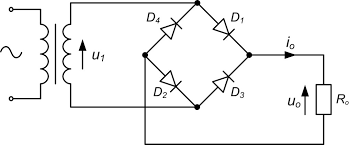
\includegraphics[width=0.8\textwidth]{8.png}
    \caption{Schemat prostownika mostkowego (Graetza).}
    \label{fig:schemat_mostek}
\end{figure}

\section*{Wyniki i obliczenia}

\subsection*{Pomiar}

\begin{itemize}
    \item \textbf{Bez kondensatora:} napięcie wyjściowe: 0 -- 504 mV
    \item \textbf{Z kondensatorem:} napięcie: 352 -- 400 mV
\end{itemize}
\begin{figure}[H]
    \centering
    \begin{subfigure}{0.45\textwidth}
        \centering
        \includegraphics[width=\linewidth]{9.png}
        \caption{Odczyt pomiaru bez kondensatora.}
        \label{fig:schemat1}
    \end{subfigure}
    \hfill
    \begin{subfigure}{0.45\textwidth}
        \centering
        \includegraphics[width=\linewidth]{10.png}
        \caption{Odczyt pomiaru z kondensatorem.}
        \label{fig:schemat2}
    \end{subfigure}
    \caption{Porównanie odczytów z oraz bez kondensatora.}
    \label{fig:porownanie}
\end{figure}

\subsection*{Teoretyczne obliczenia}

\[
I_{dc} = \frac{2 \cdot I_m}{\pi}
\]

\[
P_{dc} = I_{dc}^2 \cdot R_L = \left( \frac{2 \cdot I_m}{\pi} \right)^2 \cdot R_L
\]

\[
I_{rms} = \frac{I_m}{\sqrt{2}}
\]

\[
P_{ac} = I_{rms}^2 \cdot (r_f + R_L) = \left( \frac{I_m}{\sqrt{2}} \right)^2 \cdot (r_f + R_L)
\]

gdzie $r_f$ jest rezystancją diody, na stronie producenta podane $0{,}6\ \Omega$, w naszych obliczeniach przyjmiemy $1\ \Omega$.

\subsection*{Obliczona sprawność}
\[
\eta = \frac{P_{dc}}{P_{ac}} \cdot 100\% = 0{,}812 \left( 1 + \frac{r_f}{R_L} \right) \cdot 100\% = 0{,}812 \left( 1 + \frac{1\,\Omega}{100000\,\Omega} \right) \cdot 100\% \approx 81{,}2\%
\]

\section*{3. Dyskusja błędów}

Otrzymane wyniki pomiarów były zgodne z teorią. Podczas pomiarów korzystaliśmy z oscyloskopu, którego dokładność zależy m.in. od ustawionej czułości, próbki i rodzaju przebiegu. W przypadku szybko zmieniających się sygnałów, takich jak napięcie wyjściowe prostowników, trudniej było jednoznacznie odczytać wartość napięcia średniego.

Możliwe były także drobne zakłócenia na przebiegach oraz błędy odczytu związane z ręcznym odczytywaniem wartości z wykresów. Mimo to, ogólny charakter działania prostowników został zachowany i pomiary były wystarczająco dokładne do porównania z teorią.

\section*{4. Wnioski}

Podczas ćwiczenia zbadano działanie trzech rodzajów prostowników: jednopołówkowego, dwupołówkowego z odczepem środkowym oraz mostkowego. Otrzymane przebiegi i napięcia średnie były zbliżone do wartości teoretycznych, co potwierdziło poprawność działania układów.

Pomiary potwierdziły działanie prostowników zgodne z przewidywaniami, a różnice mogły wynikać z błędów pomiarowych i charakterystyki użytych elementów.
\section*{5. Protokół}
\begin{figure}[H]
    \centering
    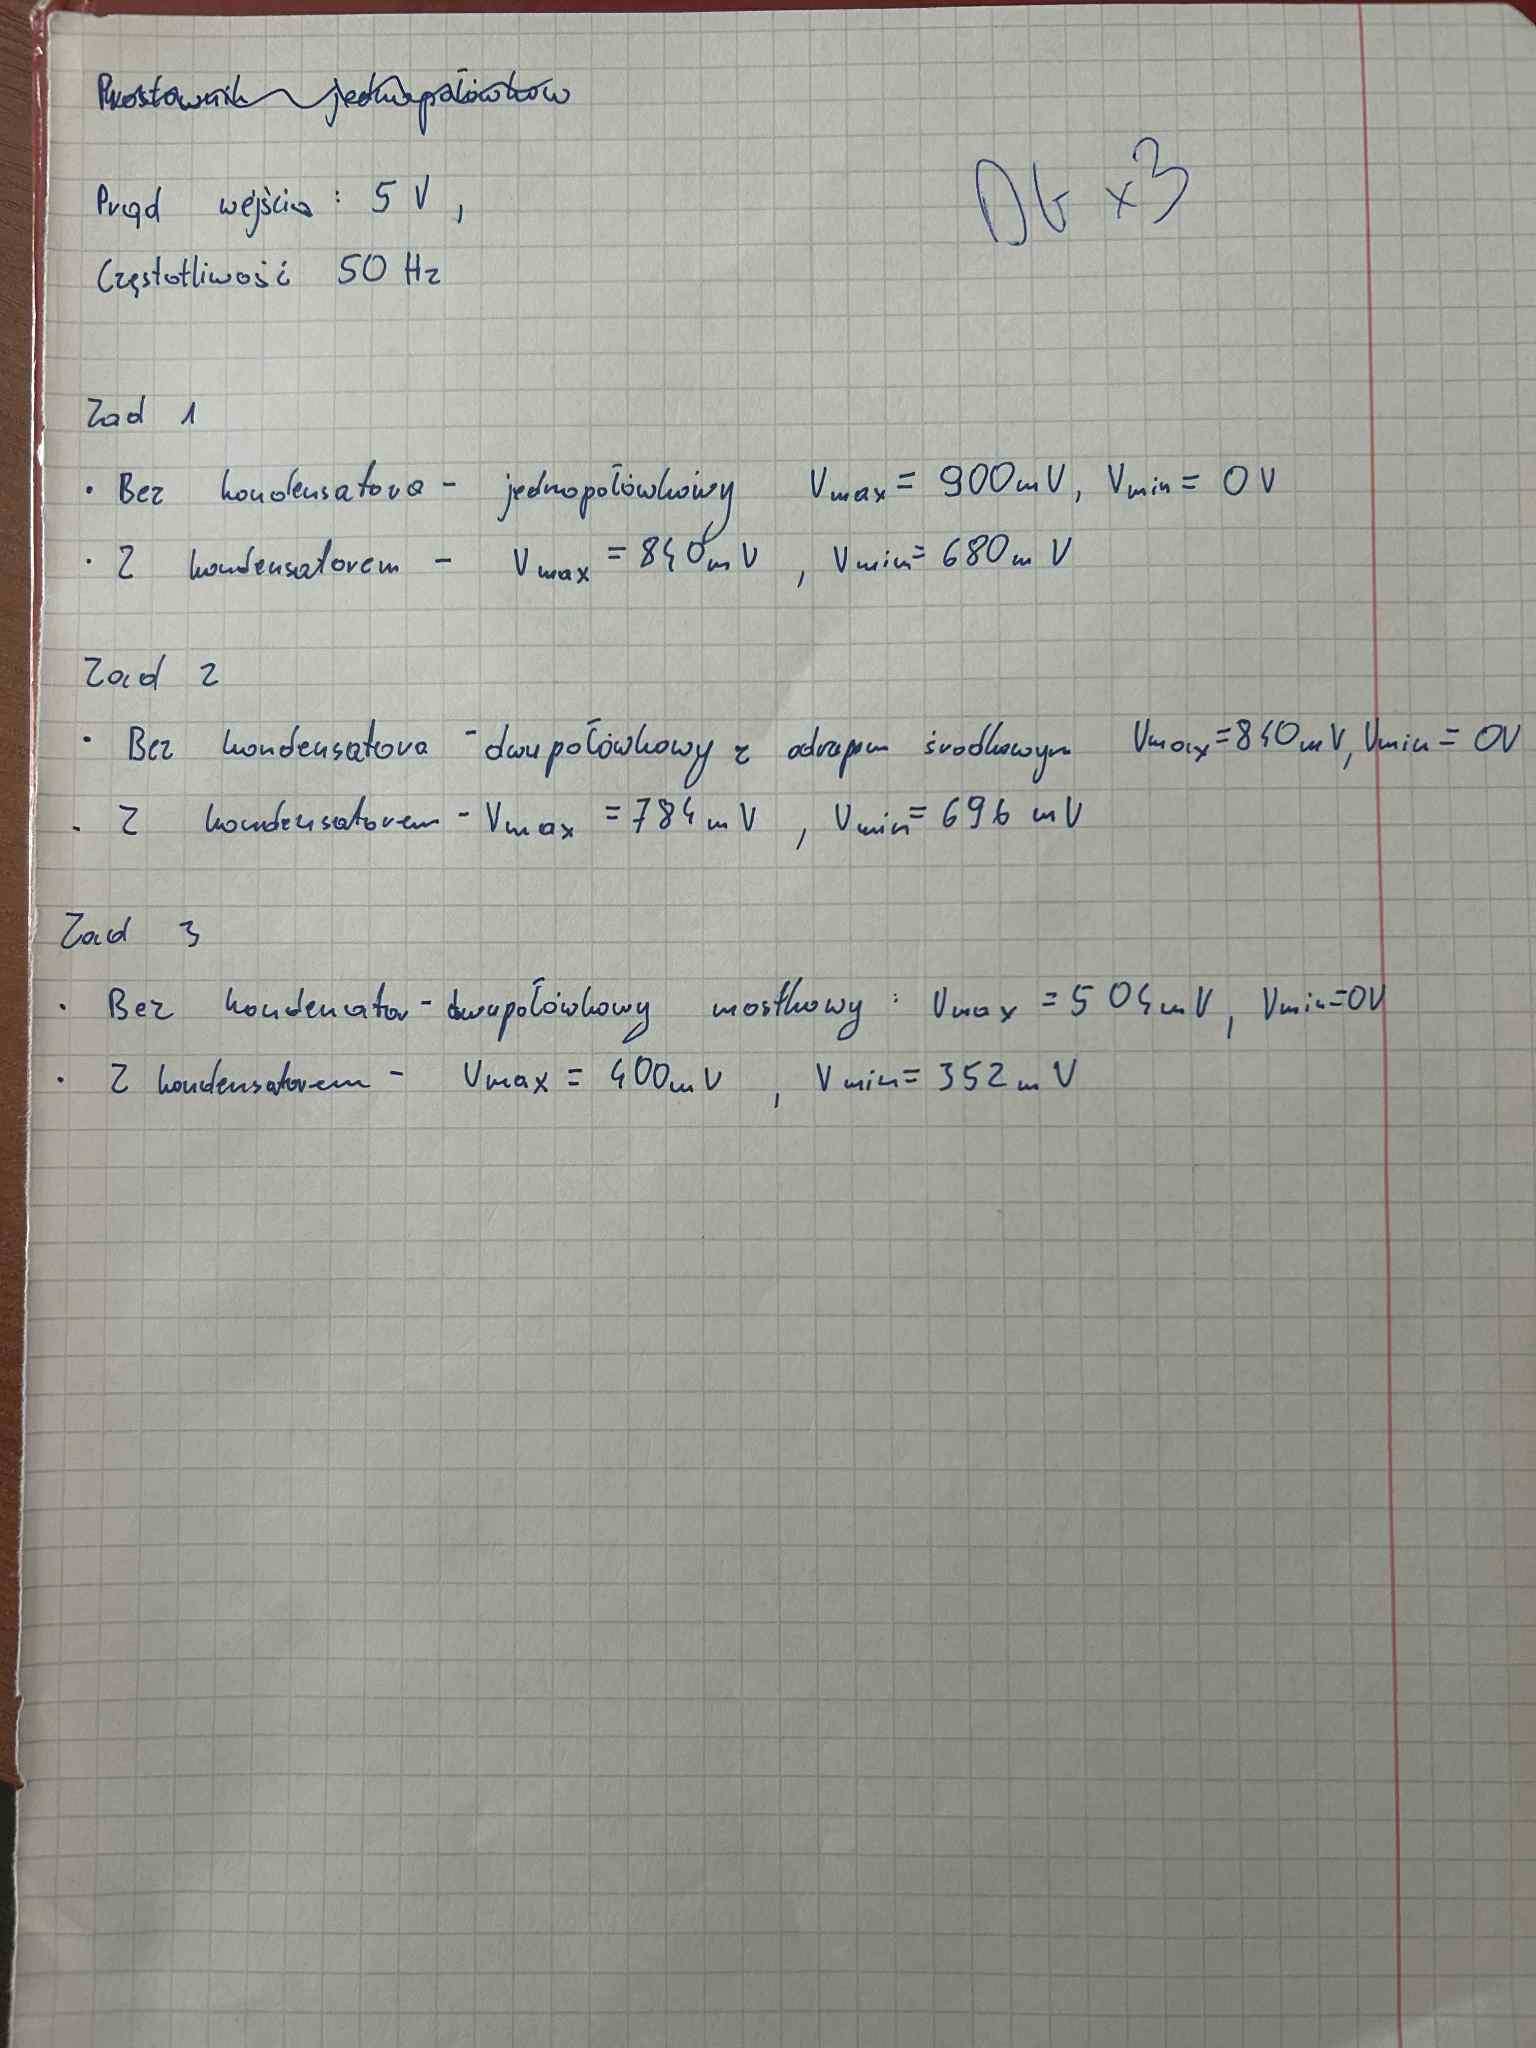
\includegraphics[width=0.8\textwidth]{11.jpg}
    \caption{Protokół.}
    \label{fig:schemat_dwu}
\end{figure}
\end{document}
